%! Author = t
%! Date = 4/28/24

% Preamble
\documentclass[11pt]{article}

% Packages
\usepackage{amsmath}
\usepackage{titlesec}
\usepackage{enumitem}

\usepackage{float}
\usepackage{multirow}
\usepackage{makecell}
\usepackage{tabularx}
\usepackage{array, adjustbox, booktabs, pgffor}
\usepackage{xparse}
\usepackage{graphicx}
\newcolumntype{C}[1]{>{\centering\arraybackslash}p{#1}}

\titleformat{\section}[hang]{\fontsize{20}{24}\selectfont\filcenter}{\Roman{section}}{1em}{}

\title{Networks Assignment\\ Chapter 5}
\author{Braiko Timofei\\1820243088}
\date{\today}
\maketitle
\newpage

% Document
\begin{document}
    \section{Task}\label{sec:task-1}
    Explain the difference between routing, forwarding, and switching.

    \subsection{Solution}
    \begin{itemize}
        \item \textbf{Routing} - Process responsible for filling and updating routing tables;
        makes a decision which router to use.
        \item \textbf{Forwarding} - Decides what to do after packet arrives.
        \item \textbf{Switching} - Process of switching packets between devices on the same network
    \end{itemize}
    \newpage


    \section{Task}\label{sec:task-2}
    For the network given in Fig 5-1, give global distance–vector tables like Table 5-1 (where D is the
    distance, N is neighbor) when
    \begin{enumerate}
        \item Each node knows only the distances to its immediate neighbors
        \item Each node has reported the information it had in the preceding step to its immediate neighbors.
        \item Step (2) happens a second time.
    \end{enumerate}

    \begin{center}
        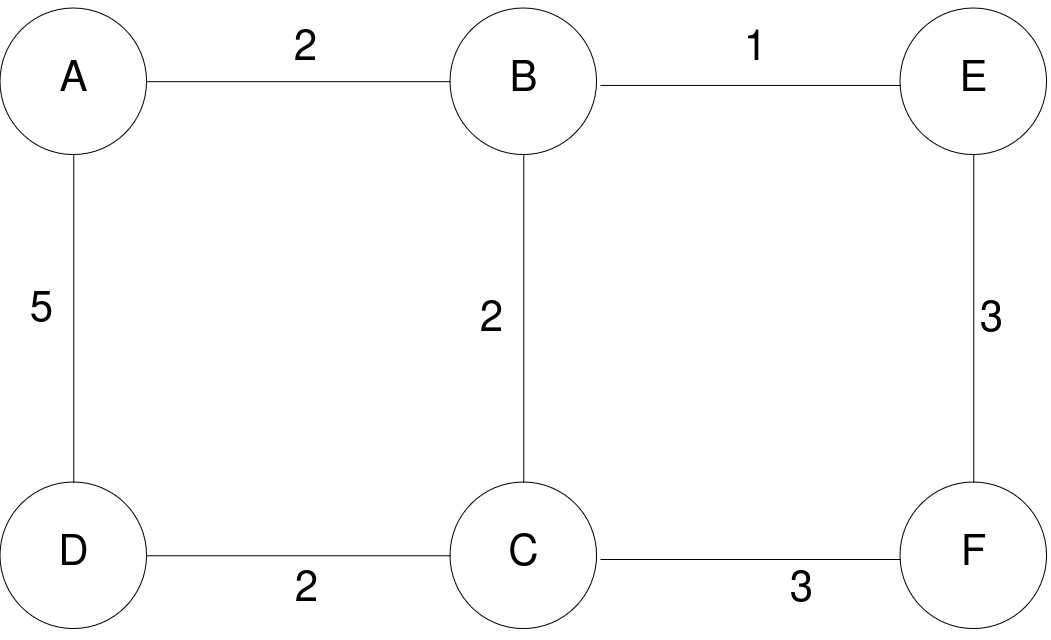
\includegraphics[width=0.6\textwidth]{figs/graph}
    \end{center}

    \subsection{Solution}


    \begin{table}[H]
        \begin{adjustbox}{center}
            \begin{tabular}{|c|C{0.7cm}|C{0.7cm}||C{0.7cm}|C{0.7cm}||C{0.7cm}|C{0.7cm}||C{0.7cm}|C{0.7cm}||C{0.7cm}|C{0.7cm}||C{0.7cm}|C{0.7cm}|}
                \hline
                & \multicolumn{12}{|c|}{Distances and neighbours to each node} \\ \cline{2-13}
                Node & \multicolumn{2}{|c||}{A} & \multicolumn{2}{|c||}{B} & \multicolumn{2}{|c||}{C} & \multicolumn{2}{|c||}{D} & \multicolumn{2}{|c||}{E} & \multicolumn{2}{|c|}{F} \\ \cline{2-13}
                & D & N & D & N & D & N & D & N & D & N & D & N &
                \hline
                A & 0 & -- & 2 & B & ? & -- & 5 & D & ? & -- & ? & -- &
                B & 2 & A & 0 & -- & 2 & C & ? & -- & 1 & E & ? & -- &
                C & ? & -- & 2 & B & 0 & -- & 2 & D & ? & -- & 3 & F &
                D & 5 & A & ? & -- & 2 & C & 0 & -- & ? & -- & ? & -- &
                E & ? & -- & 1 & B & ? & -- & ? & -- & 0 & -- & 3 & F &
                F & ? & -- & ? & -- & 3 & C & ? & -- & 3 & E & 0 & -- &
                \hline
            \end{tabular}\label{tab:table-a}
        \end{adjustbox}
        \caption{Solution to point 1}
    \end{table}


    \begin{table}[H]
        \begin{adjustbox}{center}
            \begin{tabular}{|c|C{0.7cm}|C{0.7cm}||C{0.7cm}|C{0.7cm}||C{0.7cm}|C{0.7cm}||C{0.7cm}|C{0.7cm}||C{0.7cm}|C{0.7cm}||C{0.7cm}|C{0.7cm}|}
                \hline
                & \multicolumn{12}{|c|}{Distances and neighbours to each node} \\ \cline{2-13}
                Node & \multicolumn{2}{|c||}{A} & \multicolumn{2}{|c||}{B} & \multicolumn{2}{|c||}{C} & \multicolumn{2}{|c||}{D} & \multicolumn{2}{|c||}{E} & \multicolumn{2}{|c|}{F} \\ \cline{2-13}
                & D & N & D & N & D & N & D & N & D & N & D & N &
                \hline
                A & 0 & -- & 2 & B & 4 & B & 5 & D & 3 & B & 6 & E &
                B & 2 & A & 0 & -- & 2 & C & 4 & C & 1 & E & 4 & E &
                C & 4 & B & 2 & B & 0 & -- & 2 & D & 3 & B & 3 & F &
                D & 5 & A & 4 & C & 2 & C & 0 & -- & ? & -- & 5 & C &
                E & 3 & B & 1 & B & 3 & B & ? & -- & 0 & -- & 3 & F &
                F & ? & -- & 4 & E & 3 & C & 5 & C & 3 & E & 0 & -- &
                \hline
            \end{tabular}\label{tab:table-b}
        \end{adjustbox}
        \caption{Solution to point 2}
    \end{table}


    \begin{table}[H]
        \begin{adjustbox}{center}
            \begin{tabular}{|c|C{0.7cm}|C{0.7cm}||C{0.7cm}|C{0.7cm}||C{0.7cm}|C{0.7cm}||C{0.7cm}|C{0.7cm}||C{0.7cm}|C{0.7cm}||C{0.7cm}|C{0.7cm}|}
                \hline
                & \multicolumn{12}{|c|}{Distances and neighbours to each node} \\ \cline{2-13}
                Node & \multicolumn{2}{|c||}{A} & \multicolumn{2}{|c||}{B} & \multicolumn{2}{|c||}{C} & \multicolumn{2}{|c||}{D} & \multicolumn{2}{|c||}{E} & \multicolumn{2}{|c|}{F} \\ \cline{2-13}
                & D & N & D & N & D & N & D & N & D & N & D & N &
                \hline
                A & 0 & -- & 2 & B & 4 & B & 5 & D & 3 & B & ? & -- &
                B & 2 & A & 0 & -- & 2 & C & 4 & C & 1 & E & 4 & E &
                C & 4 & B & 2 & B & 0 & -- & 2 & D & 3 & B & 3 & F &
                D & 5 & A & 4 & C & 2 & C & 0 & -- & 5 & B & 5 & C &
                E & 3 & B & 1 & B & 3 & B & 5 & C & 0 & -- & 3 & F &
                F & 6 & B & 4 & E & 3 & C & 5 & C & 3 & E & 0 & -- &
                \hline
            \end{tabular}\label{tab:table-c}
        \end{adjustbox}
        \caption{Solution to point 3}
    \end{table}


    \newpage
    \section{Task}\label{sec:task-3}
    Suppose we have the forwarding tables shown in Table 5-2 for nodes A and F in a network where all
    links have cost 1.
    Give a diagram of the smallest network consistent with these tables.

    \subsection{Solution}

     \begin{center}
        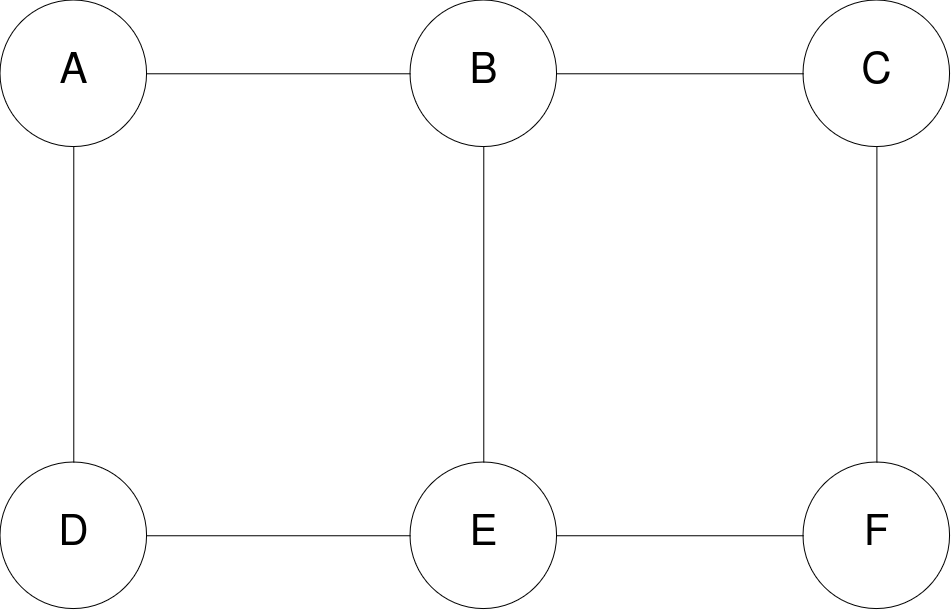
\includegraphics[width=0.6\textwidth]{figs/task3}
    \end{center}
     \newpage


    \section{Task}\label{sec:task-4}
    An unfragmented IP packet, shown in Fig 5-2(a), has 1400 bytes of data and a 20-byte IP header.
    When the packet arrives at router RA, which has an MTU of 532 bytes, it has to be fragmented.
    The 3 fragmented packets are shown in Fig 5-2(b).
    Suppose these fragments all pass through another router RB with an MTU of 380 bytes, not counting the link header
    \begin{enumerate}
        \item Show the fragments the router RB produced.
        \item If the packet were originally fragmented for this MTU, how many fragments would be produced?
    \end{enumerate}

    \begin{center}
        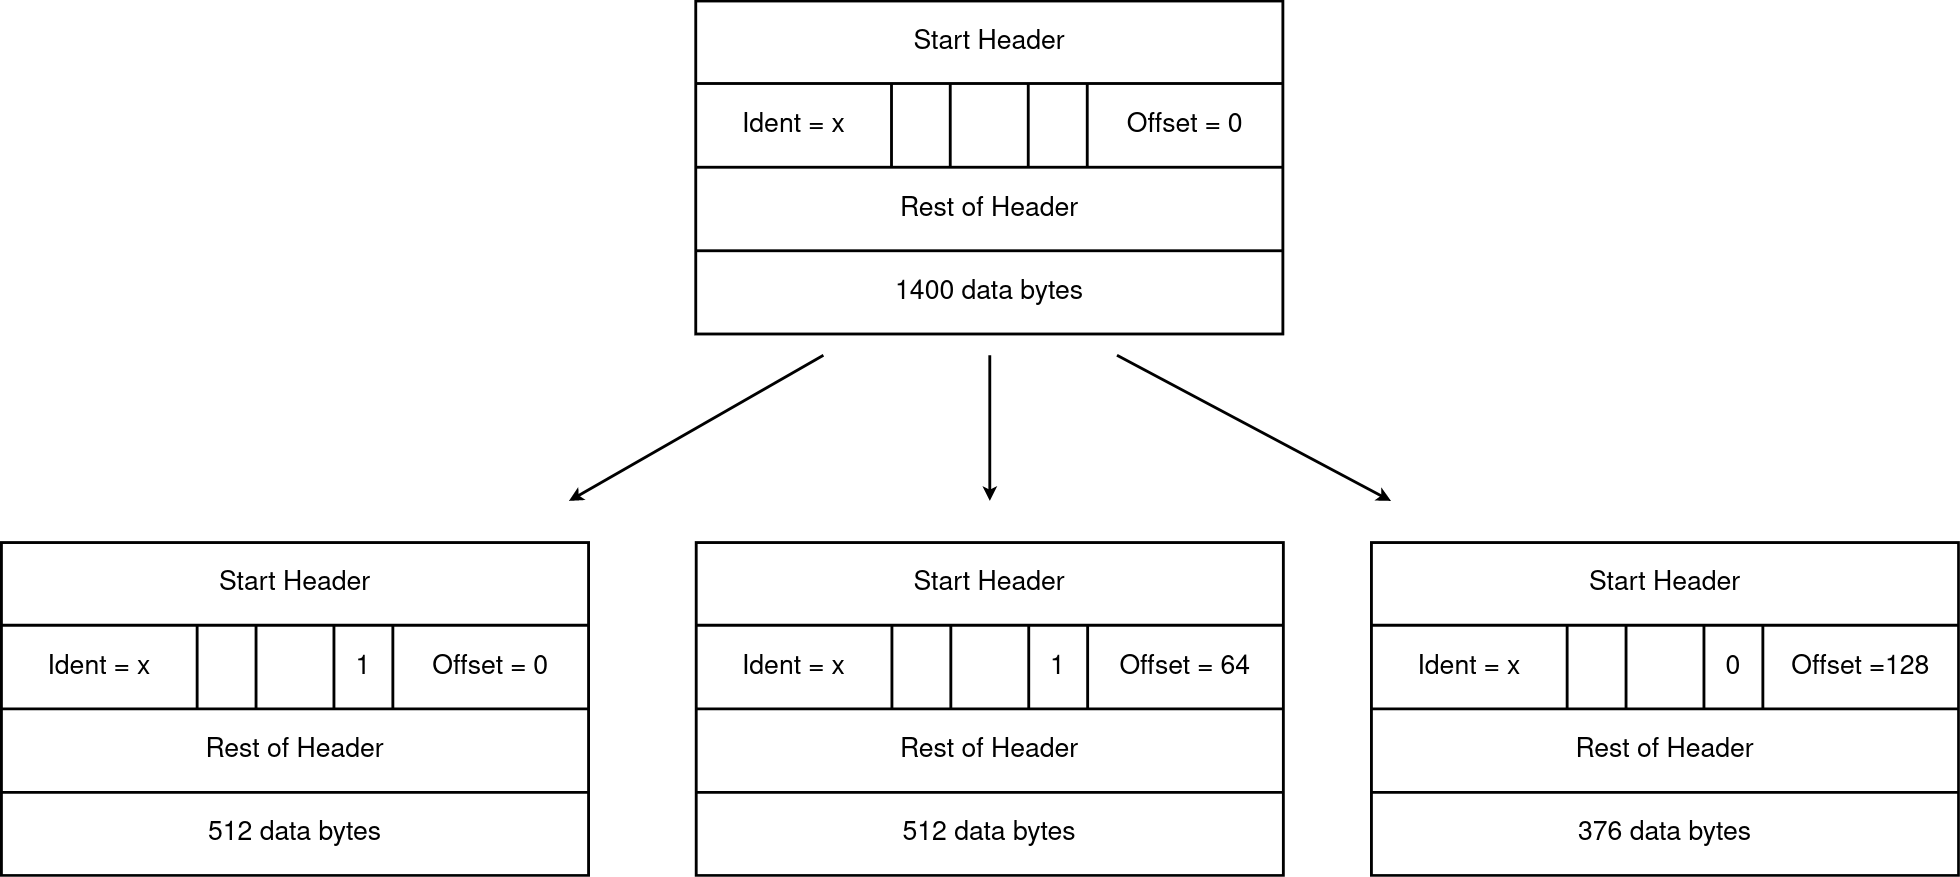
\includegraphics[width=1\textwidth]{figs/Task4}
    \end{center}

    \newpage

    \subsection{Solution}
    Internet protocol (IP) uses nontransparent fragmentation process to pass packets via routers.
    Hence, it treats each fragmented packet as original packet and does not reassemble fragments at intermediate routers.

    \paragraph{1.} After router RB receives first and second fragmented packets, it treats them separately and
    divides each of them to two smaller packets.
    Third packet is less than MTU of RB. Therefore, it is transmitted the same as it was.
    In total, router RB transmits 5 packets.

    \begin{center}
        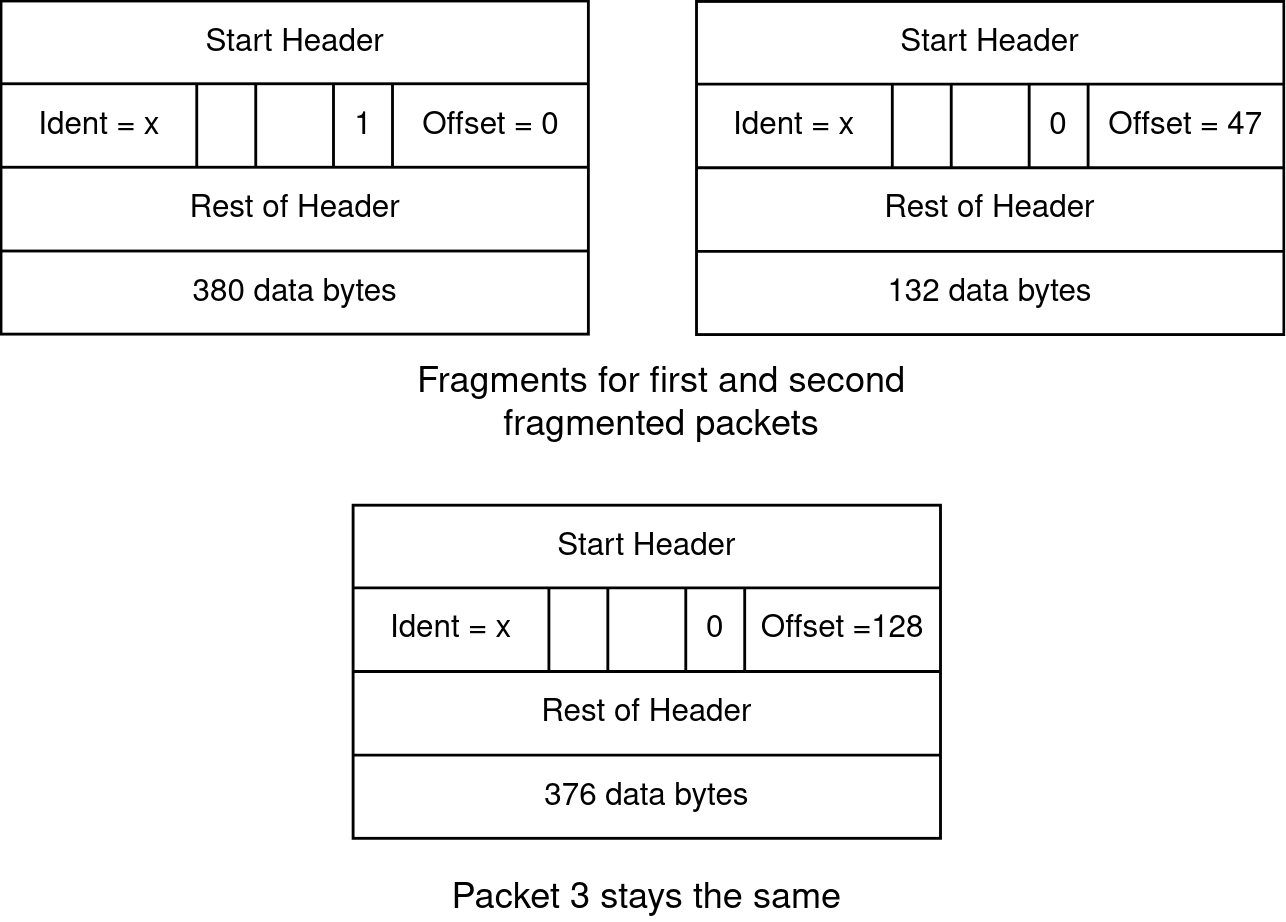
\includegraphics[width=0.85\textwidth]{figs/Sol4-1}
    \end{center}

    \paragraph{2.}
    The initial packet size is 1400 bytes.
    Thus, if it was directly send to router RB, the number of packets would be:
    $1400/380 \approx 3.6 = 4$ packets.
    \newpage


    \section{Task}\label{sec:task-5}
    What is the maximum bandwidth at which an IP host can send 576-byte packets
    without having the Ident field wrap around within 60 seconds?
    Suppose that IP’s maximum segment lifetime (MSL) is 60 seconds;
    that is, delayed packets can arrive up to 60 seconds late but no later.
    What might happen if this bandwidth were exceeded?

    \subsection{Solution}
    IP packets contain Ident field with 16 bits len.
    So in total we have $2^{16}$ unique Indents.
    As they shouldn't be repeated during transmission, we obtain the following formulas:

    \begin{subequations}
        \begin{equation}
            \frac{576 * 2^{16} * 8}{60} \approx 5033164.8 \hspace{4} bps
        \end{equation}

        \begin{equation}
            5033164.8 \hspace{4} bps = 629145.6 \hspace{4} Bps = 614.4 \hspace{4} KiBps
        \end{equation}
    \end{subequations}

    \paragraph{Answer:} 614 KiBps
    \newpage


    \section{Task}\label{sec:task-6}
    An organization has been assigned the prefix 200.1.1.0/24 and wants to form subnets for four
    departments, with hosts as follows:
    \vspace{15}

    \begin{minipage}{.5\textwidth}
        \begin{itemize}
            \item Department A 72 hosts
            \item Department B 35 hosts
        \end{itemize}
    \end{minipage}
    \begin{minipage}{.5\textwidth}
        \begin{itemize}
            \item Department C 20 hosts
            \item Department D 18 hosts
        \end{itemize}
    \end{minipage}

    \begin{enumerate}
        \item Give a possible arrangement of subnet masks to make this possible.
        \item Suggest what the organization might do if department D grows to 34 hosts.
    \end{enumerate}

    \subsection{Solution}
    Each department has different number of supporting hosts,
    so we need to preserve enough bits in IP address for each department.

    \paragraph{1.}

    \textbf{Department A:}
    \begin{center}
        72 hosts $< 2^7 \longrightarrow$ \textbf{Range:} 200.1.1.0 -- 200.1.1.127; \textbf{Mask:} 255.255.255.0 \\
        11001000 00000001 00000001 0$\mid$xxxxxxx \\
    \end{center}

    \textbf{Department B:}
    \begin{center}
        35 $< 2^6 \longrightarrow$ \textbf{Range:} 200.1.1.128 -- 200.1.1.191; \textbf{Mask:} 255.255.255.128 \\
        11001000 00000001 00000001 10$\mid$xxxxxx \\
    \end{center}

    \textbf{Department C:}
    \begin{center}
        20 $< 2^5 \longrightarrow$ \textbf{Range:} 200.1.1.192 -- 200.1.1.223; \textbf{Mask:} 255.255.255.192 \\
        11001000 00000001 00000001 111$\mid$xxxxx\\
    \end{center}

    \textbf{Department D:}
    \begin{center}
        18 $< 2^5 \longrightarrow$ \textbf{Range:} 200.1.1.224 -- 200.1.1.256; \textbf{Mask:} 255.255.255.224 \\
        11001000 00000001 00000001 110$\mid$xxxxx \\
    \end{center}

    \begin{center}
        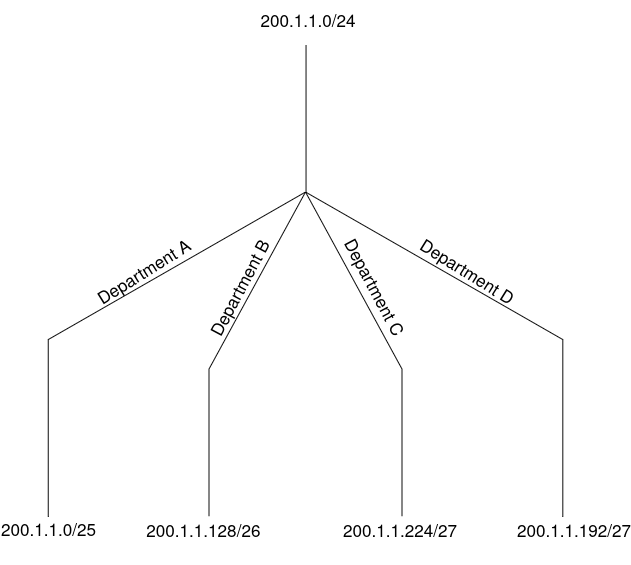
\includegraphics[width=0.75\textwidth]{figs/Sol6-1}
    \end{center}

    \paragraph{2.}
    If the number of hosts in department D increases up to 34 host, subnets should be reassigned.
    For this case, department D requires subnet with prefix '/26'.
    However, department B already takes subnet with prefix '/26' and department A with prefix '/25'.
    Therefore, there will be no subnet for department C.
    Thus, it is not possible to arrange subnets for such four department in network with prefix '/24'

    \newpage


    \section{Task}
    A router has just received the following new IP addresses: 57.6.96.0/21, 57.6.104.0/21, 57.6.112.0/21,
    and 57.6.120.0/21.
    If all of them use the same outgoing line, can they be aggregated?
    If so, to what?
    If not, why not?

    \subsection{Solution}
    Firstly, let us convert all addresses to binary format:

    \begin{center}
        \textbf{57.6.96.0/21:} 00111001 \hspace{3} 00000110 \hspace{3}01100000 \hspace{3}00000000 \\
        \textbf{57.6.104.0/21:} 00111001 \hspace{3} 00000110 \hspace{3}01110000 \hspace{3}00000000 \\
        \textbf{57.6.112.0/21:} 00111001 \hspace{3} 00000110 \hspace{3}01111000 \hspace{3}00000000 \\
        \textbf{57.6.120.0/21:} 00111001 \hspace{3}00000110 \hspace{3}01111100 \hspace{3}00000000 \\
    \end{center}

    The aggregated IP address is 57.6.96.0 with a subnet mask of /19.
    \newpage


    \section{Task}
    Given the network in Fig 5-3, determine the routing table of R2 by aggregating the routes.
    The main entries of the routing table are shown in Table 5-3.

     \begin{center}
        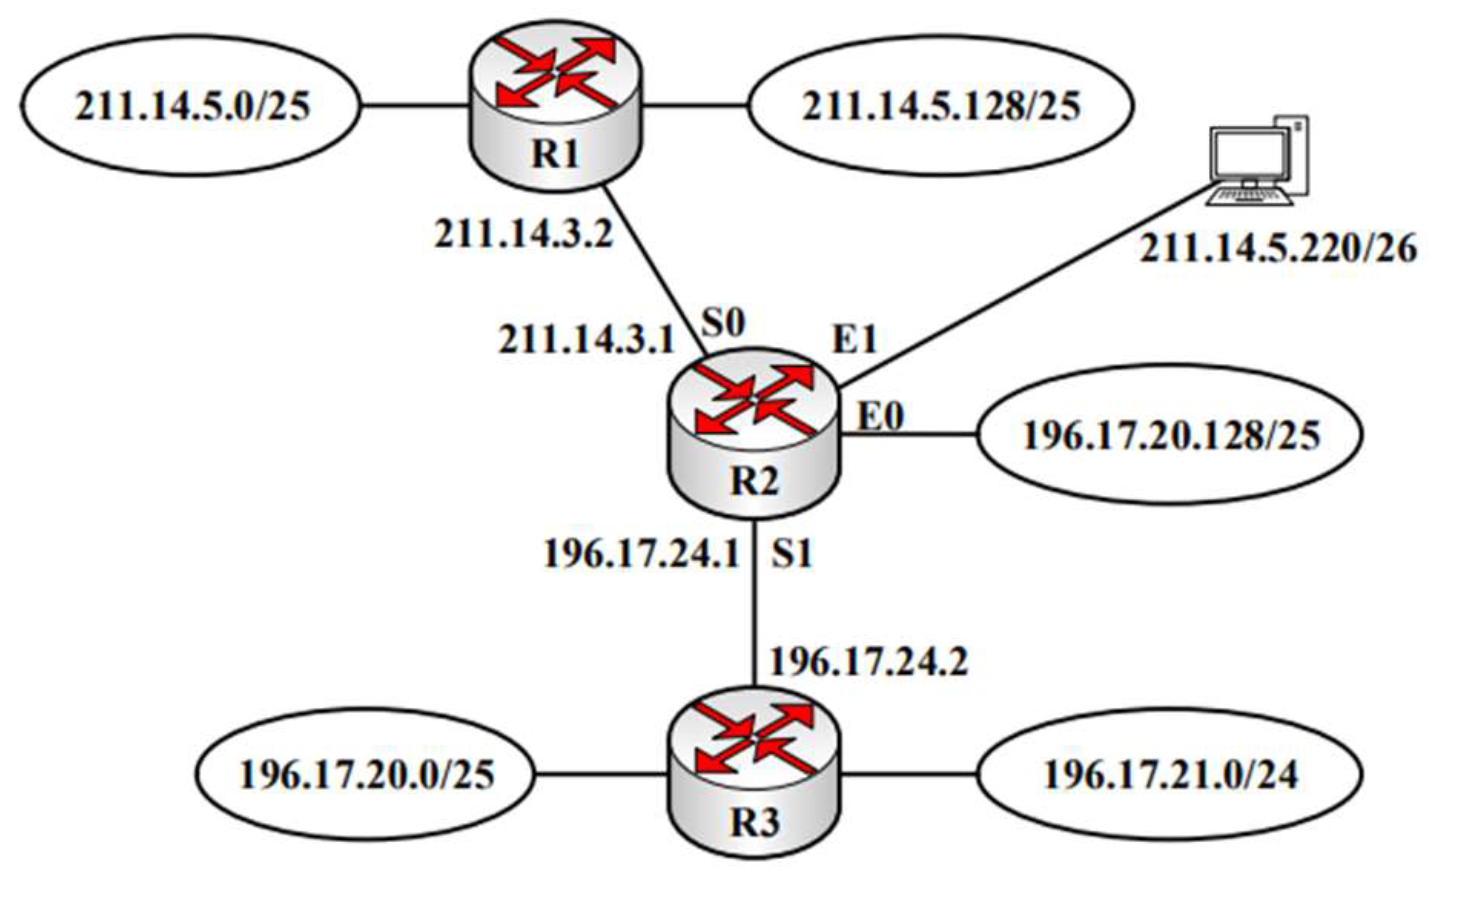
\includegraphics[width=0.75\textwidth]{figs/task8}
    \end{center}

    \subsection{Solution}

    \begin{table}[H]
        \centering
        \begin{tabular}{|c|c|c|c|c|}
            \hline
            \textbf{Destination} & \textbf{Mask} & \textbf{Next-hop} & \textbf{Interface} & \textbf{Metric} \\
            \hline
            \hline
            211.14.5.0 & 255.255.255.220 & 211.14.3.2 & S0 &  2 \\
            \hline
            211.14.5.128 & 255.255.255.220 & 211.14.3.2 & S0 & 2 \\
            \hline
            211.14.5.220 & 255.25.255.220 & Directly & E1 & 1 \\
            \hline
            196.17.20.128 & 255.255.255.220 & 196.17.20.128 & E0 & 1 \\
            \hline
            196.17.20.0 & 255.255.255.220 & 196.17.24.2 & S1 & 2 \\
            \hline
            196.17.21.0 & 255.255.255.220 & 196.17.24.2 & S1 & 2 \\
            \hline
        \end{tabular}\label{tab:table-8}
    \end{table}


\end{document}